\chapter{Learning data from a resolved liquid jet in crossflow}
	\label{ch5:jicf_resolved_simulations}



Describe here all our simulations done with JICF, what we have achieved with them, etc.

\begin{itemize}

	\item Experimental setup description
	
	\item Numerical setup description. Operating points
	
	\item Mesh convergence study
	
	\item Spray sampling
	
	\item Direct measurement of fluxes with interior boundaries
	
	\item Liquid disappearing (set levelset band ) ??
	
	\item Results:
	
		\begin{itemize}
		
			\item Breakup mechanisms
			
			\item In-nozzle phenomena of flow separation (and entrainment of gaseous bubbles)
			
			\item Spray formation and evolution with axial distance
	
		\end{itemize}
		
	\item Other results:
	
		\begin{itemize}
		
			\item Slip velocity evolution
			
			\item Vorticity distribution (horse-shoe vortices, double vortical structural in liquid)
		
		\end{itemize}

\end{itemize}

\newpage 

\section{Introduction}

The previous chapter has detailed the theory of the proposed models to build lagrangian injectors for initialising dispersed phase simulations, named Smart Lagrangian Injectors (SLI). These models, nowadays in its earliest state of maturity, are intended to be generic and applicable to a broad range of operating conditions and injector configurations. To show its capabilities, they have been developed in their first stage with resolved simulations of liquid jet in crossflow (JICF) configuration. This chapter details these simulations, performed with the software YALES2 (\textbf{ref:2011-moureau-design}). % \textbf{https://reader.elsevier.com/reader/sd/pii/S1631072110002111?token=9137B6903478D4E8E427F5D8218DFC3EB42446DB034970B14BA9DE87AA7E80D130124A7EF8D8608D21D5D465CCE05A4F&originRegion=eu-west-1&originCreation=20210524114835}

The fundamentals and the physics of non-reactive JICF have been introduced in $\S$\ref{sec:ch1_fuel_injection_technology}. This chapter shows the results, analysis and injectors obtained from a kerosene JICF simulation replicating the experimental facility tested by \citeColor[becker_breakup_2002]. This configuration is used for validating the models. Section \ref{sec:ch5_experimental_bench} displays the experimental test bench, whose numerical setup and operating conditions chosen for numerical computations are detailed in Section \ref{sec:computational_setup}.


\section{Experimental test case}
	\label{sec:ch5_experimental_bench}

\begin{figure}[h!]
	\centering
	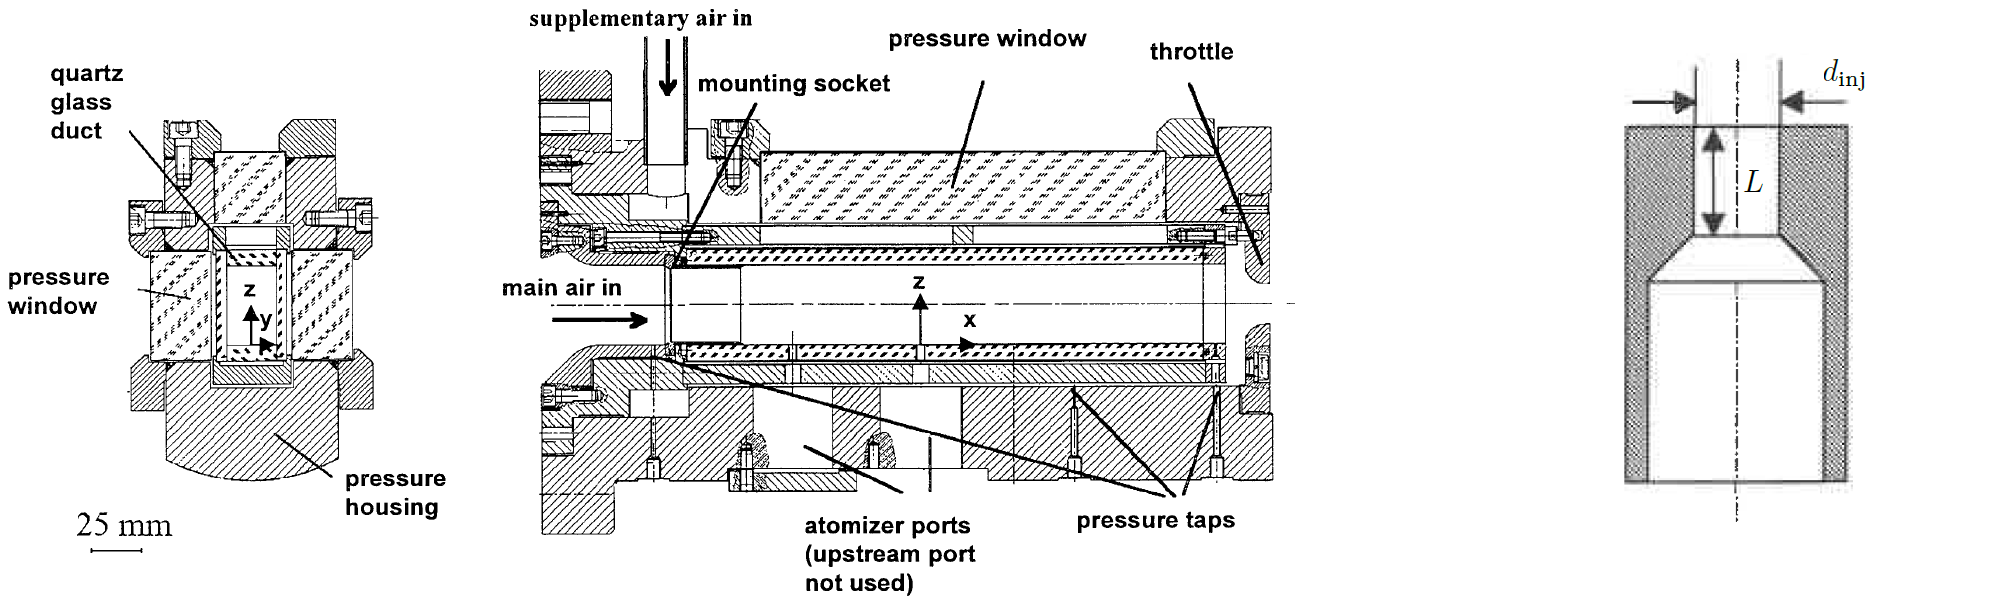
\includegraphics[scale=0.5]{./part2_developments/figures_ch5_resolved_JICF/experiment_JICF_DLR}
	\caption{\textsl{Left}: Experimental setup at DLR. \textsl{Right}: liquid nozzle geometry employed in the experimental study. Source: \citeColor[becker_breakup_2002]}
	\label{fig:experiment_JICF_DLR}
\end{figure}

Numerical simulations are validated with the experimental correlation obtained by~\cite{ref:Becker2002} for the vertical jet penetration. It has been obtained by testing experimentally several operating conditions, and has a standard deviation of value $0.81$. The correlation corresponds to the trajectory of the jet's windward side, and is given by:

\begin{equation}
    \label{eq:jicf_trajectory_becker}
    \frac{z}{d_\mathrm{inj}} = 1.57 \mathrm{q}^{0.36} \ln \left( 1 + 3.81 \frac{x}{d_\mathrm{inj}} \right)
\end{equation}

The accuracy of the mean numerical trajectories can be quantitatively assessed by defining a $L_2$ error as in Eq.~(\ref{eq:L2_JICF}): 

\begin{equation}
\label{eq:L2_JICF}
    L_2 = \sqrt{\frac{1}{N}   \sum_{i=1}^N \left( \frac{z}{d_\mathrm{inj}} \Bigr|_{\mathrm{exp},i} -   \frac{z}{d_\mathrm{inj}} \Bigr|_{\mathrm{num},i} \right)^2}
\end{equation}

\section{Computational setup}
	\label{sec:computational_setup}


\section*{Numerical domain}


\begin{figure}[ht]
     \centering
     \includeinkscape[scale=0.4]{./part2_developments/figures_ch5_resolved_JICF/DLR_becker_numerical_config}
      \caption{Numerical domain and boundary conditions of the experimental test bench of \citeColor[becker_breakup_2002]. \textsl{Left}: complete domain. \textsl{Right}: detailed view of the injection nozzle. All dimensions are in mm.}
      \label{fig:numerical_setup_maquette_JICF_DLR}
\end{figure}

\section*{Operating conditions}

%\section{YALES2 code (??)}

\section{Tools and methodologies}

\subsection{Numerical computation of jet trajectory}
	\label{sec:ch5_jicf_trajectories}

As explained in $\S$\ref{sec:ch1_fuel_injection_technology}, one of the most important features of a jet in crossflow is its trajectory. Experimental studies (\textbf{ref?}) often provide correlations for the trajectory of the windward side of the jet, such as the one from Eq. (\ref{eq:jicf_trajectory_becker}). These correlations depend on factors such as the momentum flux ratio $q$, the injection diameter $d_\mathrm{inj}$ and, in some case (\textbf{ref:Ragucci}), in the Weber number $We$. The overall dependency of the trajectory on these parameters is still unknown and an ongoing research topic.

It is therefore of interest, to obtain the trajectory for the jet penetration in the performed resolved simulations. Several methods can be used for this purpose. This section describes four possible methodologies, two based on processing instantaneous trajectories and two based on processing the mean $\psi$ field. The results obtained with these methodologies are shown in $\S$\ref{sec:results_JICF_resolved}.

\subsubsection{Methods based on instantaneous trajectories}

One possible way of obtaining tra

\begin{figure}[ht]
     \centering
     \begin{subfigure}[b]{0.45\textwidth}
         \centering
         \includeinkscape[inkscapelatex=false,scale=0.35]{./part2_developments/figures_ch5_resolved_JICF/trajectories_obtention/instantaneous_interface_3D}
         %\caption{Instantaneous jet interface}
     \end{subfigure}
     %\hfill
     \begin{subfigure}[b]{0.45\textwidth}
         \centering
         \includeinkscape[inkscapelatex=false,scale=0.35]{./part2_developments/figures_ch5_resolved_JICF/trajectories_obtention/instantaneous_interface_y0}
         %\caption{Contour of instantaneous interface at plane y = 0}
     \end{subfigure}
        \caption{\textsl{Left}: instantaneous jet interface. \textsl{Right}: contour of instantaneous interface at plane y = 0}
	% See: https://stackoverflow.com/questions/35210337/can-i-plot-several-histograms-in-3d/35225919
        \label{fig:trajectory_obtention_instantaneous_general}
\end{figure}


%\subsubsection*{Non-monotonic trajectory}

\paragraph{{Non-monotonic trajectory}}

\begin{figure}[ht]
     \centering
     \begin{subfigure}[b]{0.45\textwidth}
         \centering
         \includeinkscape[inkscapelatex=false,scale=0.35]{./part2_developments/figures_ch5_resolved_JICF/trajectories_obtention/method_a_sweep_nonMonotonic}
         %\caption{Instantaneous jet interface}
     \end{subfigure}
     %\hfill
     \begin{subfigure}[b]{0.45\textwidth}
         \centering
         \includeinkscape[inkscapelatex=false,scale=0.35]{./part2_developments/figures_ch5_resolved_JICF/trajectories_obtention/method_a_inst_trajectory}
         %\caption{Contour of instantaneous interface at plane y = 0}
     \end{subfigure}
        \caption{Obtention of non-monotonic instantaneous trajectory. \textsl{Left}: sweep process along z axis of interface points. \textsl{Right}: instantaneous trajectory.}
	% See: https://stackoverflow.com/questions/35210337/can-i-plot-several-histograms-in-3d/35225919
        \label{fig:trajectory_obtention_instantaneous_method_a}
\end{figure}


%\subsubsection*{Monotonic trajectory}
\paragraph{Monotonic trajectory}


\begin{figure}[ht]
     \centering
     \begin{subfigure}[b]{0.45\textwidth}
         \centering
         \includeinkscape[inkscapelatex=false,scale=0.35]{./part2_developments/figures_ch5_resolved_JICF/trajectories_obtention/method_b_sweep_monotonic}
         %\caption{Instantaneous jet interface}
     \end{subfigure}
     %\hfill
     \begin{subfigure}[b]{0.45\textwidth}
         \centering
         \includeinkscape[inkscapelatex=false,scale=0.35]{./part2_developments/figures_ch5_resolved_JICF/trajectories_obtention/method_b_inst_trajectory}
         %\caption{Contour of instantaneous interface at plane y = 0}
     \end{subfigure}
        \caption{Obtention of monotonic instantaneous trajectory. \textsl{Left}: sweep process along z axis of interface points, excluding points whose vertical location is lower than the vertical location of the previous ones. \textsl{Right}: instantaneous trajectory.}
	% See: https://stackoverflow.com/questions/35210337/can-i-plot-several-histograms-in-3d/35225919
        \label{fig:trajectory_obtention_instantaneous_method_b}
\end{figure}


\subsubsection{Methods based on the mean levelset field}

Another possibility to obtain mean trajectories is by using the mean field of the levelset magnitude, $\overline{\phi}$. 

\paragraph{Maximum gradient method}

This method is more similar to the experimental methods presented in \citeColor[becker_breakup_2002] and \citeColor[freitag_spray_2008], since they obtain the trajectory as the contour giving the maximum intensity gradient in the vertical direction in processed images of the mean jet.

\begin{equation}
\max \left( \nabla \overline{\phi} \right)
\end{equation}

\paragraph{Trajectory as iso-contour of mean levelset}



\subsection{Direct measurement of fluxes (interior boundaries)}
\label{subsec:ch5_interior_boundaries}

Droplet sampling is performed by tracking the center of mass of resolved structures and checking when it crosses the sampling planes. 



The sampling procedure of droplets is based on a lagrangian tracking of their center of mass. The position of the center of mass before and


\section{Results}
\label{sec:results_JICF_resolved}

\subsection{Jet topology and breakup}

\subsubsection{Effect of mesh}

\subsubsection{Effect of operating point}

\subsection{Validation with experimental trajectory}


\subsection{Spray characterization}



%\subsubsection{Sampling procedure for droplets}



\subsubsection{Droplets size distributions}

Show histograms with lognormal fit (from Lefebvre equation and from optimal fit).

\subsubsection{Definition of characteristic times}

Several characteristic times can be defined in a jet in crossflow:

\begin{itemize}

	\item Characteristic time of ligaments passage at given planes, $t_\mathrm{pas}$
	
	\item Characteristic time related to the frequency of the instabilities causing column breakup, $t_\mathrm{ins}$
	
	\item Physical definition according to ...

\end{itemize}


\subsection{Mass conservation in ACLS}

\subsection{Gaseous field and dense core characterization}
\label{subsec:ch5_dense_core_in_ACLS_simus}

\subsection{Frequential analysis}

A spectral analysis is performed to obtain the characteristic breakup frequencies. There are several ways to obtain the desired frequencies:

\begin{itemize}

	\item Use Proper Orthogonal Decomposition (POD) technique (2018 Prakash, Mukundan). This is out of the scope of this work.
	
	\item Get evolution of breakup point with time: $x_b \left( t \right)$, $z_b \left( t \right)$, then get the frequency spectrum  (2010 Wang, 2018 Prakash). Not sure we can do this with our available data, so not envisageable now.
	
	\item Locate probes along liquid column, get liquid presence rate with time. This is the one !!

\end{itemize}

\subsection{Computational performances}
\label{subsubsec:ch5_computational_performances}

%\subsection{Feeding the models (??)}
%Find a more attractive name

\subsection{Spatial discretization of sprays}

\section{Learning injectors}

\subsection{Operating point at high We}

\subsection{Operating point at low We}


\section{Conclusions}

